\documentclass[11pt]{article}
\usepackage{mystyle}
\usepackage{tikz}
\usetikzlibrary{arrows.meta}

\title{Rosen --- \S 9.4: Closures of Relations\\ \large Selected Exercises}
\author{Alston}
\date{Semester 2, 2026}

\begin{document}
\maketitle

% ======================================================================
\begin{exercise}{1}
    Let $R$ be the relation on the set $\{0, 1, 2, 3\}$ containing the
    ordered pairs $(0,1)$, $(1,1)$, $(1,2)$, $(2,0)$, $(2,2)$, and
    $(3,0)$. Find the
    \begin{enumerate}[label=(\alph*)]
        \item reflexive closure of $R$.
        \item symmetric closure of $R$.
    \end{enumerate}
\end{exercise}

% ======================================================================
\begin{exercise}{2}
    Let $R$ be the relation $\{(a,b) \mid a \neq b\}$ on the set of
    integers. What is the reflexive closure of $R$?
\end{exercise}

% ======================================================================
\begin{exercise}{3}
    Let $R$ be the relation $\{(a,b) \mid a \text{ divides } b\}$ on
    the set of integers. What is the symmetric closure of $R$?
\end{exercise}

% ======================================================================
\begin{exercise}{4}
    How can the directed graph representing the reflexive closure of
    a relation on a finite set be constructed from the directed graph
    of the relation?
\end{exercise}

% ======================================================================
\begin{exercise}{5}
    \textit{In Exercises 5--7 draw the directed graph of the reflexive
    closure of the relation with the directed graph shown.}

    \begin{center}
    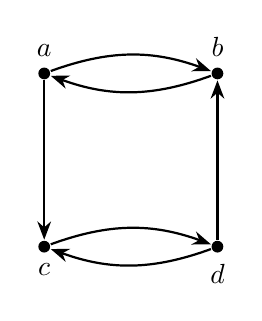
\begin{tikzpicture}[>={Stealth}, thick, scale=1.1]
        \node[circle,fill,inner sep=1.5pt,label=above:$a$] (a) at (0,2) {};
        \node[circle,fill,inner sep=1.5pt,label=above:$b$] (b) at (2,2) {};
        \node[circle,fill,inner sep=1.5pt,label=below:$c$] (c) at (0,0) {};
        \node[circle,fill,inner sep=1.5pt,label=below:$d$] (d) at (2,0) {};

        \draw[->] (a) to[bend left=20] (b);
        \draw[->] (b) to[bend left=20] (a);
        \draw[->] (c) to[bend left=20] (d);
        \draw[->] (d) to[bend left=20] (c);
        \draw[->] (a) -- (c);
        \draw[->] (d) -- (b);
    \end{tikzpicture}
    \end{center}
\end{exercise}

% ======================================================================
\begin{exercise}{6}
    \begin{center}
    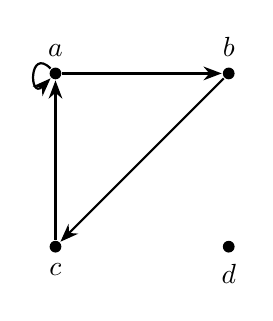
\begin{tikzpicture}[>={Stealth}, thick, scale=1.1]
        \node[circle,fill,inner sep=1.5pt,label=above:$a$] (a) at (0,2) {};
        \node[circle,fill,inner sep=1.5pt,label=above:$b$] (b) at (2,2) {};
        \node[circle,fill,inner sep=1.5pt,label=below:$c$] (c) at (0,0) {};
        \node[circle,fill,inner sep=1.5pt,label=below:$d$] (d) at (2,0) {};

        \draw[->] (a) to[out=135,in=225,looseness=8] (a);
        \draw[->] (a) -- (b);
        \draw[->] (c) -- (a);
        \draw[->] (b) -- (c);
    \end{tikzpicture}
    \end{center}
\end{exercise}

% ======================================================================
\begin{exercise}{7}
    \begin{center}
    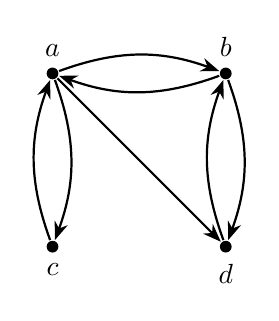
\begin{tikzpicture}[>={Stealth}, thick, scale=1.1]
        \node[circle,fill,inner sep=1.5pt,label=above:$a$] (a) at (0,2) {};
        \node[circle,fill,inner sep=1.5pt,label=above:$b$] (b) at (2,2) {};
        \node[circle,fill,inner sep=1.5pt,label=below:$c$] (c) at (0,0) {};
        \node[circle,fill,inner sep=1.5pt,label=below:$d$] (d) at (2,0) {};

        \draw[->] (a) to[bend left=20] (b);
        \draw[->] (b) to[bend left=20] (a);
        \draw[->] (a) to[bend left=20] (c);
        \draw[->] (c) to[bend left=20] (a);
        \draw[->] (b) to[bend left=20] (d);
        \draw[->] (d) to[bend left=20] (b);
        \draw[->] (a) -- (d);
    \end{tikzpicture}
    \end{center}
\end{exercise}

% ======================================================================
\begin{exercise}{8}
    How can the directed graph representing the symmetric closure of
    a relation on a finite set be constructed from the directed graph
    for this relation?
\end{exercise}

% ======================================================================
\begin{exercise}{9}
    Find the directed graphs of the symmetric closures of the
    relations with directed graphs shown in Exercises 5--7.
\end{exercise}

% ======================================================================
\begin{exercise}{10}
    \textit{Recall (Example 2): $R = \{(a,b) \mid a > b\}$ on the set
    of positive integers.}

    Find the smallest relation containing the relation in Example 2
    that is both reflexive and symmetric.
\end{exercise}

% ======================================================================
\begin{exercise}{11}
    Find the directed graph of the smallest relation that is both
    reflexive and symmetric that contains each of the relations with
    directed graphs shown in Exercises 5--7.
\end{exercise}

% ======================================================================
\begin{exercise}{12}
    Suppose that the relation $R$ on the finite set $A$ is represented
    by the matrix $M_R$. Show that the matrix that represents the
    reflexive closure of $R$ is $M_R \vee I_n$.
\end{exercise}

\end{document}